\documentclass[a4paper,12pt]{article}
\usepackage[pdftex]{graphicx}
\usepackage[magyar]{babel}
\usepackage[T1]{fontenc}
\usepackage[utf8]{inputenc}
\usepackage{multirow}
\usepackage{dcolumn}
\newcolumntype{d}[1]{D{.}{\cdot}{#1} }
\usepackage{indentfirst}
\usepackage{amsmath}
\usepackage{t1enc}
%\usepackage{epsfig}
%\usepackage{epstopdf}
\usepackage{multirow}
\usepackage{float}
\usepackage{wrapfig}
\usepackage{enumerate}
\usepackage{caption}
\usepackage{subcaption}
\usepackage{color}
\usepackage{array}
\usepackage{bbold}
\usepackage{chngpage}
\bibliographystyle{unsrt}
\usepackage[top=4cm ,bottom=4cm ,left=3cm ,right=3cm]{geometry}
%\usepackage{a4wide}
\linespread{1.3}
\usepackage{xcolor}
%\usepackage{hyperref}
%\hypersetup{hidelinks}


\DeclareGraphicsExtensions{.pdf,.eps,.png,.jpg,.mps,.gif}
\addtolength{\hoffset}{-1cm}
\addtolength{\textwidth}{2cm}
\addtolength{\voffset}{-1cm}

\pdfminorversion=5
\pdfobjcompresslevel=2
\newcommand{\celsius}{ ^\circ C } % °C
\newcommand{\megj}[1]{\textit{\small{Megjegyzés: #1}}}
\newenvironment{bfigure}[1]{    \begin{figure}[#1]
                        \begin{bf}}
                        {\end{bf}
                                \end{figure}}
\newcommand{\icaption}[1]{\caption{\textit{\textmd{#1}}}}
\newcommand{\brref}[1]{(\ref{#1}. ábra)}
\newcommand{\sz}[1]{\emph{#1. szakasz}}
\newcommand{\cg}[1]{   {\color{green}  #1 }   }
\newcommand{\vect}[1]{\boldsymbol{#1}}
\newcommand{\dd}{\mathrm{d}}

\begin{document}
        \begin{titlepage}
\author{\\ Katona Dávid  \\
Nagy Dániel \\
Szigeti Balázs \\\\\\
Fizika BSc 4. félév\\
Szerda délelőtti csoport\\\\
}

\title{\textsc{9. mérés} \\
\huge{\textbf{Elektronspin-rezonancia}\\
\vspace{10pt}\textsc{JEGYZŐKÖNYV}}}
\date{Mérés ideje:\\2017. március 8. \\
}

\centering
\maketitle
        \thispagestyle{empty}

\begin{figure}[h!]
\centering

\includegraphics[scale=0.05]{eltelogo}
\end{figure}

\small{MODERN FIZIKA LABORATÓRIUM}
%\vspace{\stretch{1}}
        \end{titlepage}

\newpage
%\tableofcontents   %tartalomjegyzék
%\newpage
%%\pagestyle{myheadings}
%\newpage

\section{A mérés célja}

A mérésünk a célja, hogy az elektronspinrezonancia-spekturmának megmérésével. Meghatározzuk a Mn és Cr ionok giromágneses-faktorát, és a hiperfinom kölcsönhatási együtthatókat. Illetve ezen felül meghatározzuk a mintában lávő atomok számát. 

\section{Mérésleírás}

\subsection{Elméleti leírás}

Az ESR mérés alapja, hogy Zeeman-felhadást hozunk létre sztatikus mágneses tér s
egítségével. Ekkor a létrejött Zeeman-alnívók elektromágneses hullám segítségével  átmeneteket hozunk létre.

A mérés során a $B_0$ sztatikus mágneses tér mellett alkalmazunk egy$ B_1 sin(2*\pi \nu t)$ oszcilláló mágneses teret, amely az átmeneteket hozunk létre. 

Az abszorpció feltétele:

\begin{equation}
h \nu = g \mu_{B}(B_0 + A m_I)
\end{equation}

Amelyben $h$ a Planck-állandó, g az ún. g-faktor, $\mu_B$ a Bohr-magneton. A a finomszerkezeti állandó, és $m_I$ a mágneses kvantumszám. 

A mérés során $B_0$ értékét változtattuk és annak a függvényében mért az abszorpciót. Megközelítőleg a mintára eső teljesítmény 10mW nagyságú volt, amelynél kisebb teljesítmény esetében a rendszernek elég ideje lett volna a relaxációra, nagyobb teljesítmény esetében pedig telítés jött volna létre a rendszerben. Emiatt kiegyenlítődés jött volna létre.

A mérésnél, hogy ki tudjuk emelni a zajból a kicsiny jeleket, ezért lock in technikát alkalmazunk, amely abból áll, hogy egy időben jól definiált periodikus változásunk és ennek segítségével kiszűrjük az így változó komponenst. Ennél a mérésnél a $B_0$ -t szinuszosan megmoduláljuk 100kHz-cel. 

A lock in technika következtében az ESR-jel derivált alakú lesz.

\subsection{Mérési eszközök}

\begin{itemize}
\item Elektronspinrezonancia-spektroszkóp
\item Számítógép
\item Mn Cr minták
\end{itemize}

\section{Adatok és kiértékelés}

A hiperfinom kölcsönhatás miatt az ESR-jel annyi volnalra esik szét, ahányféleképpen a magspin beállhat a külső térhez képest. Tehát ha a I a magspin, akkor 2I+1 féleképpen történhet meg.

\subsection{Króm}

A természetben krómnak három stabil izotópja fordul elő a $Cr^{52}$, $Cr^{53}$, illetve $Cr^{54}$. Ezek közül $Cr^{52}$ a leggyakoribb a fellelhető természetes króm megközelítőleg 83 százalékát alkotja. 

\begin{table}[h!]
\begin{center}
\begin{tabular}{|c|c|c|c|c|c|c|c|}
 \hline
$a$ & $s$ & $x_0$ & $c$ \\ \hline
$17524 \pm 455.7$ & $0.610 \pm 0.024$ & $3438.50 \pm 0.0497$ & $100 \pm 22.55$  \\ \hline
\end{tabular}
\caption{A $Cr$-minta esetében mért ESR jelre illesztett görbe paraméterei}
\label{tab:3}
\end{center}
\end{table}

A Lorentz-görbe a következő alakú:
\[  f(x) = \frac{a}{(1+s(x-x_0)^2)}\]

A $lock in$ detektálás miatt a jel derivált alakú lesz. 

Ennek deriváltját illesztjük a csúcsokra.
\[ \frac{df}{dx} = \frac{-2as(x-x_0)}{(1+s(x-x_0)^2)^2}\]

A mérés során felvettük a teljes spektrumot, illetve az egyes csúcsokat egyenként külön-külön.

A Cr-mintában lévő atomok számát ismerjük: $N_{Cr} = 8,3 * 10^{13}$, a Cr-minta csúcsok alatti területből és a Mn-csúcsok alatti összterületből meghatározható Mn-atomok száma.

Illetve ezenfelül ismerjük a Cr g-faktorát is, melynek értéke: 

\begin{equation}
g_{Cr}=1.98 \pm 0.0001
\end{equation} 

A minta a $Cr^{52}$ mellett tartalmaz megközelítőleg 1/5 arányban $Cr^{53}$-t is. Emiatt a középső nagy csúcs mellett megjelenik négy kisebb csúcs is a spektrumban.

A zaj miatt a 4 kisebb csúcs helye nem határozható meg pontosan. Ezért csak a középső csúcsra illesztettünk.

\begin{figure}[h!]
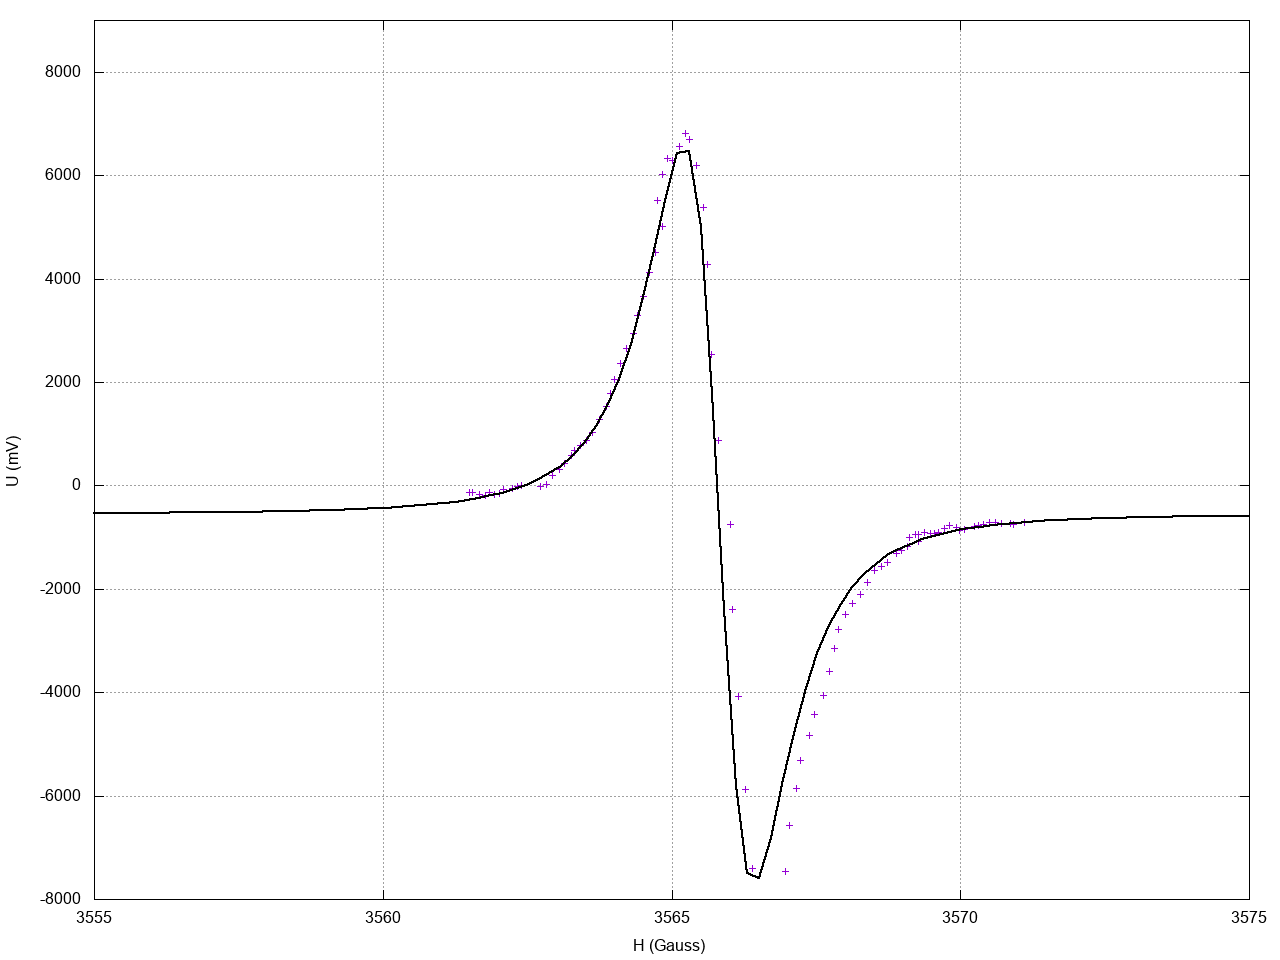
\includegraphics[width=15cm]{cr6.png}
\centering
\caption{A mérési adatok, és az illesztett derivált Lorentz-görbe Cr minta esetén}
\label{fig:4}
\end{figure}

Az izotóparányok figyelembevételével a Cr egy kis csúcsa 1/36-od területű a nagy csúcshoz képest. Az illesztésből: 

\begin{center}
\begin{equation}
T_{Cr}^{nagy}=17524 \pm 455
\end{equation}
\end{center}

Ebből:
\begin{equation}
 T_{Cr}^{kicsi}= 486 \pm 12
\end{equation}

Ebből a foton frekvenciája: 

\begin{equation}
\nu = \dfrac{g_{Cr}*\mu_{B}*m}{h} = 9.0373 GHz
\end{equation}

\subsection{Mangán}

A mérés ezen részében a $^{55}Mn^{+2}$ mintát vizsgáljuk:

\begin{table}[h!]
\begin{center}
\begin{tabular}{|c|c|c|c|c|}
 \hline
$m$ & $a$ & $s$ & $x_0$ & $c$ \\ \hline
$-2.5$ & $12930 \pm 432.3$ & $0.812 \pm 0.023$ & $3225.00 \pm 0.0634$ & $-50 \pm 16.25$ \\ \hline
$-1.5$ & $12930 \pm 443.4$ & $0.889 \pm 0.025$ & $3290.40 \pm 0.0578$ & $-154\pm 31.28$ \\ \hline
$-0.5$ & $11930 \pm 426.2$ & $0.989 \pm 0.027$ & $3357.20 \pm 0.0582$ & $-284\pm 45.12$ \\ \hline
$0.5$  & $13050 \pm 456.1$ & $0.783 \pm 0.024$ & $3425.36 \pm 0.0332$ & $-284\pm 45.7$ \\ \hline
$1.5$  & $11924 \pm 439.1$ & $1.005 \pm 0.022$ & $3495.02 \pm 0.0435$ & $-104\pm 25.67$ \\ \hline
$2.5$  & $11524 \pm 447.2$ & $0.910 \pm 0.027$ & $3565.82 \pm 0.0523$ & $-554\pm 132.85$ \\ \hline
\end{tabular}
\caption{A $Mn$-minta esetében mért ESR jelre illesztett görbe paraméterei}
\label{tab:1}
\end{center}
\end{table}

Ezekből a számolt területek:
\begin{table}[h!]
\begin{center}
\begin{tabular}{|c|c|}
 \hline
$\textrm{mérés}$ & $T$ \\ \hline
$1$ & $(4.5079 \pm 0.02) \cdot 10^4$ \\ \hline
$2$ & $(4.3082 \pm 0.02) \cdot 10^4$ \\ \hline
$3$ & $(3.7687 \pm 0.02) \cdot 10^4$ \\ \hline
$4$ & $(4.6332 \pm 0.02) \cdot 10^4$ \\ \hline
$5$ & $(3.7367 \pm 0.02) \cdot 10^4$ \\ \hline
$6$ & $(3.7941 \pm 0.02) \cdot 10^4$ \\ \hline
\end{tabular}
\caption{A $Mn$-minta esetében a Lorentz-görbe alatti területek}
\label{tab:2}
\end{center}
\end{table}

Ha a mágneses kvantumszám függvényében ábrázoljuk a Mn illesztéséből származó csúcsok helyeit. Akkor egy lineáris függvényt kaptunk ahol:

\begin{equation}
B_0 = - \dfrac{A}{g_M \mu_B} * m_I + \dfrac{h \nu}{g_M \mu_B}
\end{equation}

Tehát a függvény meredekségéből és tengelymetszetéből meghatározhatók akívánt értékek.

\begin{figure}[h!]
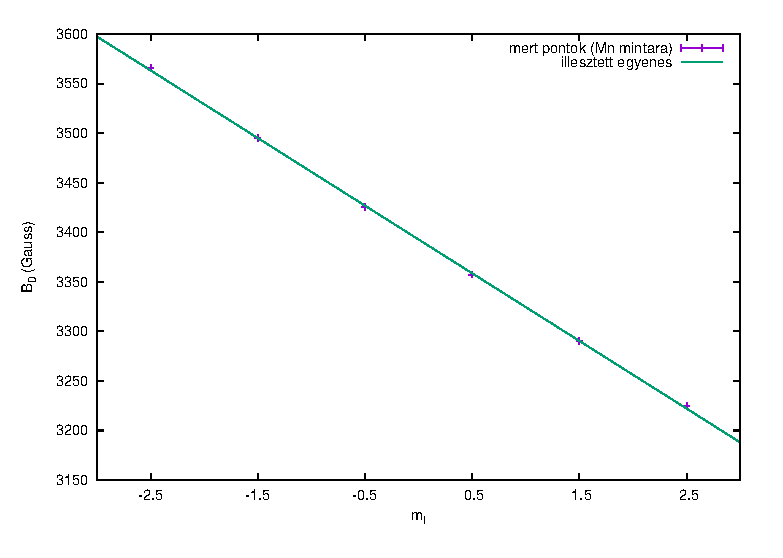
\includegraphics[width=15cm]{Mn.eps}
\centering
\caption{A mérési adatok, és az illesztett derivált Lorentz-görbe Cr minta esetén}
\label{fig:4}
\end{figure}

Az illesztéshez a gnuplot nevű programot használtuk.

Az illesztési paraméterek a következők:
\begin{equation}
a  = -68.2427 \pm 0.552    és b = 3392.66 \pm 0.8317   
\end{equation}

Ez alapján a kívánt értékek:

\begin{equation}
g_{M_n}= -\dfrac{h \nu}{\mu_{B} b}= 2.1354 \pm 0.0005
\end{equation}

\begin{equation}
A=-ag_{M_n} * \mu_{B} = (1.327 \pm 0.01) 10^{-25} J
\end{equation}

\subsubsection{Mn-atomok számának meghatározása}

A 6 csúcs alatti terület összege: $T_{M_n}$

Mivel a Cr spektrumot 1mV-os méréshatárral mértük. Ezért a területek arányát meg kell szorozni 5-tel.

\begin{center}
\begin{equation}
N_{M_n}= N_{Cr} * 5 *\dfrac{T_{M_n}}{T_{Cr}}=(5.8609 \pm 0.012) * 10^{15} J
\end{equation}
\end{center}

\end{document}